\chapter{Exam 2018}
\section{Assignment 1. App Supporting Social Exercising}
A non-profit organisation wants to provide an app to support increased exercising by facilitating social contact between users. The aim is to increase the users’ exercising by connecting them to other users who want to do the same type of exercises. 
\subsection{Assignment 1.1. System Definition}
\begin{center}
\fbox{
    \parbox{0.8\textwidth}{
        An IT‐system provided by a non‐profit organisation to support a community of users in establishing contacts to other users in the community who want to do exercises. A couple of volunteers in the non‐profit organisation will take care of system administration, but apart from that the users in the community will be the only ones applying the system. A user can set up an event that involves a specific type of exercise, e.g. running, playing football or bicycling. Other users can view the events that are available and sign up for the ones that are interesting for them. Events will have at least a single occurrence, but may also have multiple occurrences that are happening several times with defined time intervals, e.g. weekly. The aim of the system is to increase the amount of exercising for the users. The system allows users to select events, but it will also encourage users to participate in events based on their stated preferences. The system will be based on a server at the non‐profit organisation and clients on the users’ smart phones. It will be developed by a software company in collaboration with volunteers in the non‐profit organisation and prospective users.
    }
}
\end{center}
\textbf{Divide the system definition into the elements of the FACTOR criterion}
\begin{center}
    \begin{tabular}{|c|p{9cm}|}
    \hline
        \textbf{Functionality} & A user can set up an event that involves a specific type of exercise, e.g. running, playing football or bicycling. Other users can view the events that are available and sign up for the ones that are interesting for them. \\  \hline
        \textbf{Application Domain} & An IT‐system provided by a non‐profit organisation to support a community of users in establishing contacts to other users in the community who want to do exercises. A couple of volunteers in the non‐profit organisation will take care of system administration, but apart from that the users in the community will be the only ones applying the system. \\  \hline
        \textbf{Conditions} & It will be developed by a software company in collaboration with volunteers in the non‐profit organisation and prospective users.  \\  \hline
        \textbf{Technology} & The system will be based on a server at the non‐profit organisation and clients on the users’ smartphones. \\ \hline
        \textbf{Objects} & Events will have at least a single occurrence, but may also have multiple occurrences that are happening several times with defined time intervals, e.g. weekly. \\ \hline
        \textbf{Responsibility} & The aim of the system is to increase the amount of exercising for the users. The system allows users to select events, but it will also encourage users to participate in events based on their stated preferences. \\ \hline
    \end{tabular}
\end{center}
\subsubsection*{Notes}
In this particular assignment the system definition was written criteria by criteria, with regards to FACTOR. This is not always the case, assignment 3.2 in this set is of same form, however the FACTOR criteria are scrambled in the system definition. \textbf{Read and apply the system definition line by line}.\\
FACTOR criterion:
\begin{itemize}
    \item \textbf{F}unctionality: the main tasks and functionalities of the system
    \item \textbf{A}pplication Domain: the people and/or organisation that will be actively using the system
    \item \textbf{C}onditions: the conditions under which the system will be developed and used - for instance, a system is developed by an external company, which uses a third party to gather relevant information or data
    \item \textbf{T}echnology: the technologies that will be used during development, and for/by the system
    \item \textbf{O}bjects: the most important objects in the system
    \item \textbf{R}esponsibility: the general purpose of the system
\end{itemize}
\begin{center}
    \rule{10cm}{.4pt}
\end{center}
The system developers describe the problem domain as follows:
\begin{itemize}
    \item The community is made up of users who have registered in the system
    \item A user can create an event
    \item An event happens at least once, in which case there is exactly one event occurrence for the event
    \item An event may also be repeated, in which case there are several event occurrences for the event 
    \item A user can sign up to participate in an event occurrence
\end{itemize}

\begin{figure}[H]
    \centering
    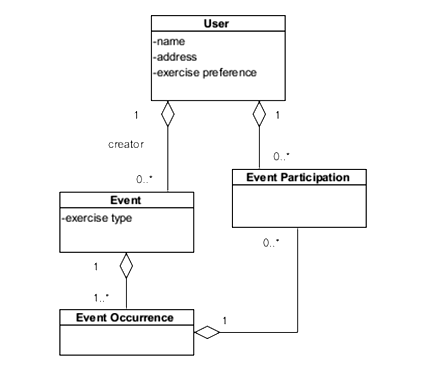
\includegraphics[width=0.75\textwidth]{figures/assignment1-2classdiagram2018.png}
\end{figure}

The system developers have also described the behaviour of the problem domain as follows:
\begin{itemize}
    \item A user can join the community by registering in the system
    \item A user can leave the community whenever he wants to by registering that in the system 
    \item A user can create events, where each has a specific exercise type
    \item After an event is created, the user creates one or more event occurrences, where each has a date, time and place 
    \item A user can sign up for event occurrences that are created by other users; and cancel the signup if he decides that 
    \item The users who have signed up for an event occurrence can participate when the event occurrence happens 
    \item Users can rate an event occurrence they have participated in (after it has happened)
    \item After an event occurrence is created, it can be opened for signup; at this time, other users may sign up and cancel their signups 
    \item At a point in time, signup will be closed and other users can no longer sign up or cancel
    \item When the first event occurrence of an event has happened, it is not possible to create further event occurrences 
    \item When all event occurrences have happened, the event and all its event occurrences as well as all the open user participations will be marked as completed 
    \item A user participation starts with the user signing up for an event occurrence; then the user can either participate or cancel 
    \item If a user leaves the community, all his open user participations will be marked as completed 
\end{itemize}
\subsection{Assignment 1.2. Event Table}
The table below lists all events in the problem domain. For each event in the table, mark which problem domain classes it is related, using a ‘+’ (for sequence and selection) or an ‘*’ (for iteration): 
\begin{center}
    \begin{tabular}{|l|c|c|c|c|}
    \hline
         & User & Event & Event Occurrence & Event Participation \\ \hline
        user registered & + & & &  \\ \hline
        user left community & + & & & *  \\ \hline
        event created & & + & &  \\ \hline
        event occurrence created & * & * & + &  \\ \hline
        event occurrence happened & & * & + &  \\ \hline
        event completed & & + & + & +  \\ \hline
        sign-up opened & & & + &  \\ \hline
        sign-up closed & & & + &  \\ \hline
        user signed up & * & & * & +  \\ \hline
        user sign-up cancelled & * & & * & + \\ \hline
        user participated & * & & & + \\ \hline
        event occurrence rated & * & & * & + \\ \hline
    \end{tabular}
\end{center}
\subsubsection*{Notes}
\textbf{+} denotes that the event affects the object zero or one time, while \textbf{*} denotes zero or more times.

\subsection{Assignment 1.3. Statechart}
Make a statechart diagram for each of the four classes in the class diagram above.

\begin{figure}[H]
    \centering
    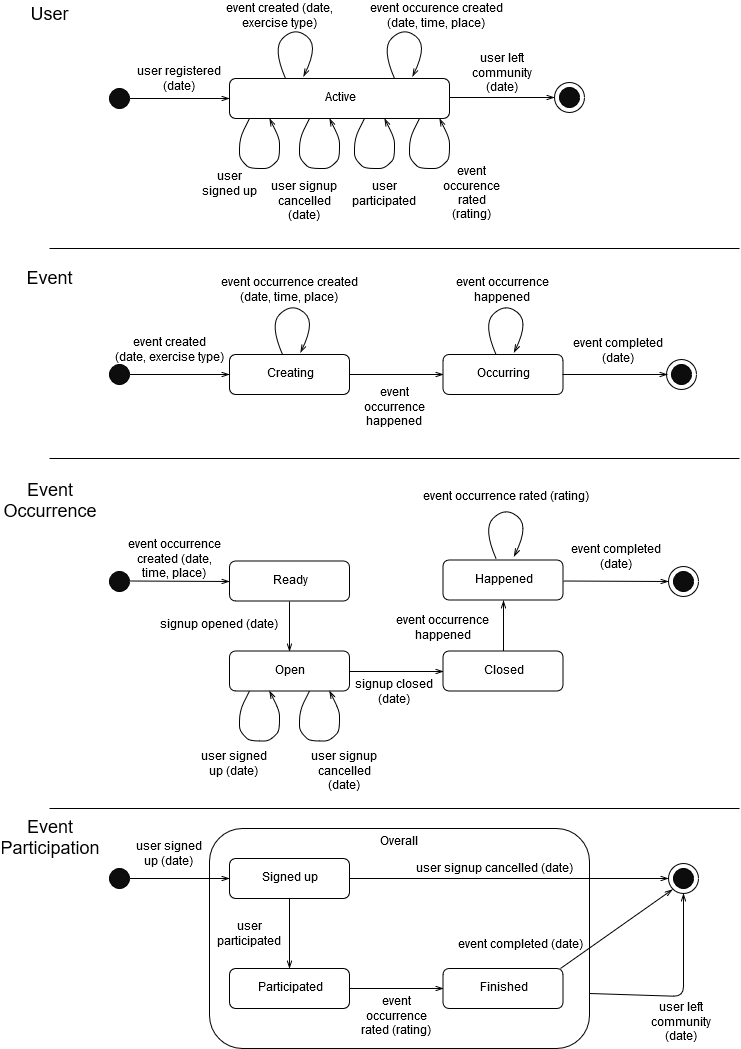
\includegraphics[width=\textwidth]{figures/assignment1-3statechartdiagrams2018.png}
\end{figure}


\section{Assignment 2. Object-Oriented Concepts}
\subsection{Assignment 2.1. Define what a class is}
A description of a collection of objects sharing structure, behavioural pattern, and attributes.

\subsection{Assignment 2.2. Define what an object is}
An entity with identity, state and behaviour.

\subsection{Assignment 2.3. Explain the relation between class and object}
An object is created from the description of a class. An object belongs to a class (from which it was created). Each class contains a set of objects; we refer to them as the objects of the class.

\section{Assignment 3. Truck Fleet Monitoring}
\begin{center}
\fbox{
    \parbox{0.8\textwidth}{
        A company operates a fleet of large trucks. The trucks are transporting containers for the company’s customers. The company wants a system to monitor its fleet of trucks. The purpose of the system is to monitor the position of each truck as well as where the driver of the truck is in solving a specific task. A task is to move one or more containers from an origin X to a destination Y. A task is defined by a customer in collaboration with the company’s sales department. When a task is to be carried out, a dispatcher in the company makes one or more assignments to the task. A single assignment is to transport one container from X to Y, and it has one truck as well as one or two drivers allocated to carry out the assignment. The system must provide information about the trucks and drivers assigned to a task and who the drivers of each truck are; it must also provide information about the time when an assignment started, when it is expected to be completed and when it is actually completed; it must also provide information about the specific container that an assignment involves. The system will be developed by an external software company, and the sales department, the dispatcher and the drivers will be involved in the development. The sales department and dispatcher will use PCs connected to a centralised server in the company’s headquarter. Each driver will have a mobile computer that helps him get an overview of the task and report back to the headquarter on task progress.
    }
}
\end{center}
\subsection{Assignment 3.1. Problem Domain and Application Domain Objects}
Which of the following objects belong either to the Problem Domain (PD), Application Domain (AD), both domains (PD and AD), or none of the domains (neither PD nor AD): 
\begin{center}
    \begin{tabular}{|l|c|c|c|c|}
    \hline
         & PD & AD & PD \& AD & Neither  \\ \hline
        Company             & & x & & \\ \hline
        Truck               & x & & & \\ \hline
        Customer            & x & & & \\ \hline
        Container           & x & & & \\ \hline
        Sales department    & & x & & \\ \hline
        Dispatcher          & & x & & \\ \hline
        Driver              & & & x & \\ \hline
        Task                & x & & & \\ \hline
        Server              & & & & x \\ \hline
        Mobile Computer     & & x & & \\ \hline
    \end{tabular}
\end{center}
\subsubsection*{Notes}
Problem Domain is being watched by Application Domain. Users use Application domain to watch Problem Domain. Problem Domain is any kind of data in the application.
\subsection{Assignment 3.2. System Definition}
Make a system definition divided into the six elements of the FACTOR criterion.
\begin{center}
    \begin{tabular}{|c|p{10cm}|}
    \hline
        \textbf{Functionality}: & The company wants a system to monitor its fleet of trucks. A task is defined by a customer in collaboration with the company’s sales department. When a task is to be carried out, a dispatcher in the company makes one or more assignments to the task. The system must provide information about the trucks and drivers assigned to a task and who the drivers of each truck are; it must also provide information about the time when an assignment started, when it is expected to be completed and when it is actually completed; it must also provide information about the specific container that an assignment involves. \\ \hline
        \textbf{Application Domain} & A company operates a fleet of large trucks. The trucks are transporting containers for the company’s customers. Truck drivers on assignment, dispatchers, and the sales department \\ \hline
        \textbf{Conditions} & The system will be developed by an external software company, and the sales department, the dispatcher and the drivers will be involved in the development. \\ \hline
        \textbf{Technology} & The sales department and dispatcher will use PCs connected to a centralised server in the company’s headquarter. Each driver will have a mobile computer that helps him get an overview of the task and report back to the headquarter on task progress. \\ \hline
        \textbf{Objects} & A task is to move one or more containers from an origin X to a destination Y.  A single assignment is to transport one container from X to Y, and it has one truck as well as one or two drivers allocated to carry out the assignment. \\ \hline
        \textbf{Responsibility} & The purpose of the system is to monitor the position of each truck as well as where the driver of the truck is in solving a specific task. \\ \hline
    \end{tabular}
\end{center}
\subsection{Assignment 3.3. Class Diagram}
Make a class diagram of the problem domain of this system. The classes must have the relevant attributes.

\begin{figure}[H]
    \centering
    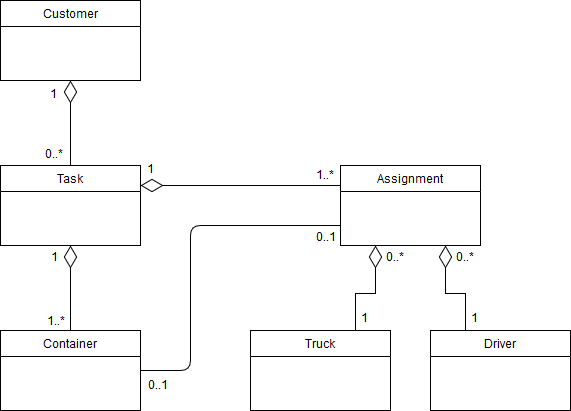
\includegraphics[width=0.75\textwidth]{figures/assignment3-3classdiagram2018.png}
\end{figure}

\subsection{Assignment 3.4. System Architecture}
Design the system architecture of the system.
\begin{itemize}
    \item Select the architectural pattern(s) that is/are relevant for the system:
    \begin{itemize}
        \item Generic Architecture and Client-Server Architecture with distributed data
    \end{itemize}
    \item Explain the reason for this selection:
    \begin{itemize}
        \item The generic architecture is chosen as a basis for clients and server. There is no fixed number of clients and they are geographically dispersed, so the client-server architecture is chosen. Distributed data is chosen such that a driver and monitor and report about a task if there is no connection to the server.
    \end{itemize}
    \item Make a diagram with the component architecture for the system. You can disregard the technical platform.
\end{itemize}


\begin{figure}[H]
    \centering
    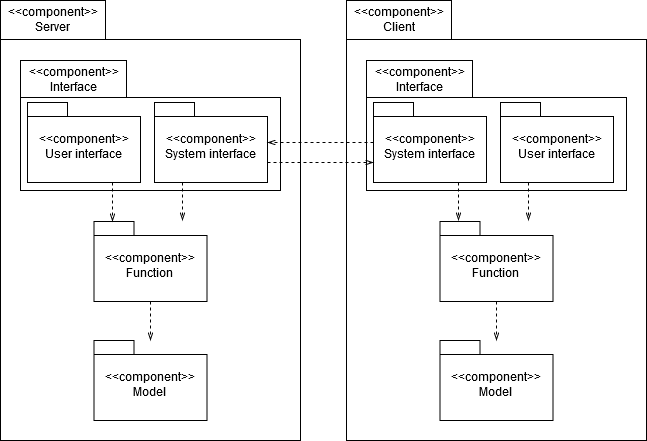
\includegraphics[width=0.85\textwidth]{figures/assignment3-4componentarchitecture2018.png}
\end{figure}

\subsubsection*{Notes}
Architectural patterns are found in sections 10.2 and 10.3 on pages 194-203 in \ad. 

\section{Assignment 4. Web Shop for Wine Club}
A wine club is selling wine through its web shop to a group of customers who are members of the club. A Customer can join the club and thereby becomes an active member. Eventually, the Customer may leave the club. In the meantime, while the Customer is active, he can order wine from the club. \\
Below is the class diagram for the problem domain. 

\begin{figure}[H]
    \centering
    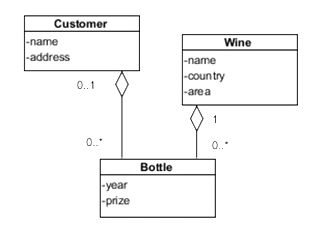
\includegraphics[width=0.5\textwidth]{figures/assignment4classdiagram2018.png}
\end{figure}

\subsection{Assignment 4.1. Patterns}
Which of the following patterns are used in the class diagram above:
\begin{itemize}
    \item \sout{The role pattern}
    \item (The relation pattern)
    \item (The hierarchy pattern)
    \item The item-descriptor pattern
    \item \sout{The stepwise relation pattern}
    \item \sout{The stepwise role pattern}
    \item \sout{The composite pattern}
\end{itemize}
\subsubsection*{Notes}
The relation pattern (between Customer and Wine) and hierarchy pattern (between Customer and Bottle) are not obvious answers, but are accepted as such.
\begin{center}
    \rule{10cm}{.4pt}
\end{center}
Below are the statechart diagrams for the classes in the problem domain.

\begin{figure}[H]
    \centering
    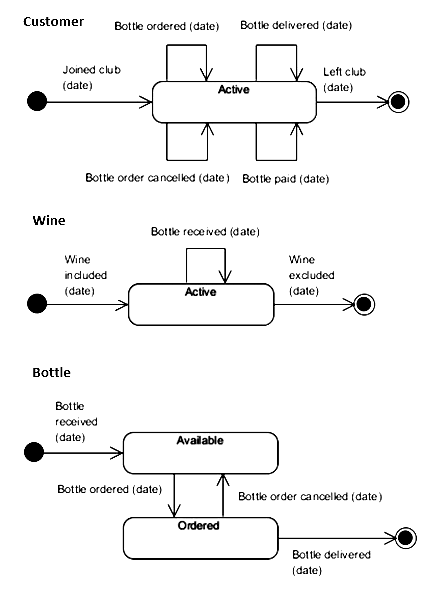
\includegraphics[width=0.65\textwidth]{figures/assignment4statechart2018.png}
\end{figure}

\subsection{Assignment 4.2. Behaviour}
Make an event table for this problem domain.
\begin{center}
    \begin{tabular}{|l|c|c|c|}
    \hline
         & Customer & Wine & Bottle \\ \hline
        joined club (date) & + & & \\ \hline
        left club (date) & + & & \\ \hline
        bottle ordered (date) & * & & * \\ \hline
        bottle delivered (date) & * & & + \\ \hline
        bottle paid (date) & * & & \\ \hline
        bottle order cancelled (date) & * & & * \\ \hline
        wine included (date) & & + & \\ \hline
        wine excluded (date) & & + & \\ \hline
        bottle received (date) & & * & + \\ \hline
    \end{tabular}
\end{center}
\subsubsection*{Notes}
Classes are gathered from the class diagram, and events are gathered from statechart diagrams.
\subsection{Assignment 4.3. Model Component}
Simple solution:
\begin{figure}[H]
    \centering
    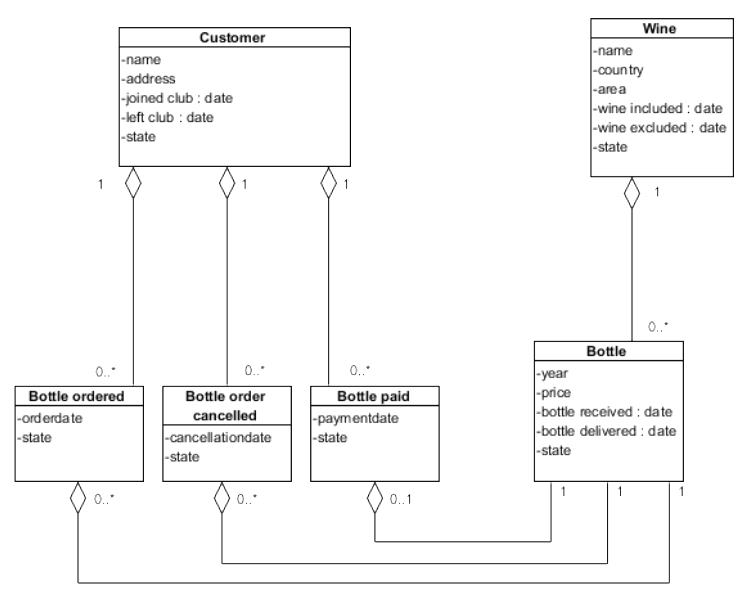
\includegraphics[width=0.5\textwidth]{figures/assignment4-3modelcomponent2018-1.png}
\end{figure}
\noindent Enhanced solution:
\begin{figure}[H]
    \centering
    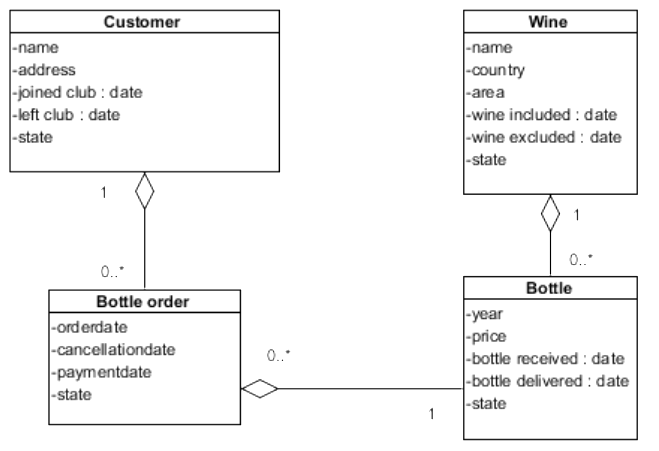
\includegraphics[width=0.5\textwidth]{figures/assignment4-3modelcomponent2018-2.png}
\end{figure}

\subsubsection*{Notes}
The above is an enhanced solution. A more simple solution, in which the three date fields of the Bottle order are abstracted to each their event, is also accepted.